\documentclass[aspectratio=169,14pt]{beamer}
\usetheme{default}
\usepackage{fontspec}
\setmainfont{texgyrepagella-regular.otf}[BoldFont=texgyrepagella-bold.otf,ItalicFont=texgyrepagella-italic.otf,BoldItalicFont=texgyrepagella-bolditalic.otf]
\setsansfont{texgyreheros-regular.otf}[BoldFont=texgyreheros-bold.otf,ItalicFont=texgyreheros-italic.otf,BoldItalicFont=texgyreheros-bold.otf,BoldItalicFeatures={FakeSlant=0.2}]
\setmonofont{lmmono10-regular.otf}[Scale=0.85]
\setbeamertemplate{navigation symbols}{}
\usepackage{pgfpages}
\newif\ifpresenter
\ifdefined\PresenterVersion\presentertrue\else\presenterfalse\fi
\ifpresenter
  \setbeameroption{show notes on second screen=right}
  \setbeamertemplate{note page}[plain]
\fi
\usepackage{amsmath,amssymb,bm,booktabs,array,graphicx,xcolor}
\usepackage{tikz,pgfplots,adjustbox,listings,xurl}
\pgfplotsset{compat=1.18}
\usetikzlibrary{arrows.meta,positioning,calc,fit,shapes.geometric,decorations.pathreplacing,patterns}
% UIUC official brand colors, verified 2026-10-23.
% https://brand.illinois.edu/visual-identity/color
\definecolor{IlliniOrange}{HTML}{FF5F05}
\definecolor{IlliniBlue}{HTML}{13294B}
\definecolor{Storm}{HTML}{707372}
\definecolor{LightStorm}{HTML}{C6C7C6}
\definecolor{Industrial}{HTML}{1D58A7}
\definecolor{Patina}{HTML}{007E8E}
\tikzset{>=Stealth, every node/.style={font=\small,text=IlliniBlue}, box/.style={draw=IlliniBlue,rounded corners=2pt,align=center,inner sep=6pt,execute at begin node=\hyphenpenalty10000\relax}, orangebox/.style={box,draw=IlliniOrange,very thick}, edge/.style={->,thick,IlliniBlue}, accent/.style={->,very thick,IlliniOrange}}
\pgfplotsset{every axis/.append style={width=13.5cm,height=6.5cm,axis line style={IlliniBlue},tick label style={font=\small,text=IlliniBlue},label style={font=\small,text=IlliniBlue},legend style={font=\small,draw=none,fill=white},grid style={LightStorm},major grid style={LightStorm},axis lines=left,clip=false}, every axis plot/.append style={thick}}

\definecolor{slidepaper}{RGB}{234,220,201}
\setbeamercolor{background canvas}{bg=slidepaper}
\setbeamercolor{normal text}{fg=IlliniBlue}
\setbeamercolor{frametitle}{fg=IlliniBlue}
\setbeamercolor{title}{fg=IlliniBlue}
\setbeamercolor{item}{fg=IlliniOrange}
\setbeamerfont{frametitle}{size=\large,series=\bfseries}
\setbeamerfont{title}{size=\Large,series=\bfseries}
\setbeamertemplate{itemize item}{\color{IlliniOrange}$\bullet$}
\setbeamertemplate{itemize subitem}{\color{IlliniOrange}\footnotesize$\circ$}
\setbeamercolor{orangerule}{bg=IlliniOrange}
\setbeamertemplate{headline}{\begin{beamercolorbox}[wd=\paperwidth,ht=0.1cm,dp=0.1cm]{orangerule}\end{beamercolorbox}}
\setbeamertemplate{footline}{\begin{beamercolorbox}[wd=\paperwidth,ht=0.1cm,dp=0.1cm]{orangerule}\end{beamercolorbox}}
\setbeamersize{text margin left=0.65cm,text margin right=0.65cm}
\setlength{\leftmargini}{1.1em}
\newenvironment{slidebullets}{\begin{itemize}\setlength\itemsep{0.8em}}{\end{itemize}}
\pgfplotsset{every axis/.append style={legend style={fill=slidepaper}}}
\lstdefinelanguage{CoursePython}{keywords={from,import,for,in,if,else,def,return,assert,True,False,None},sensitive=true,morecomment=[l]{\#},morestring=[b]',morestring=[b]"}
\lstset{language=CoursePython,basicstyle=\ttfamily\small,keywordstyle=\color{IlliniBlue}\bfseries,commentstyle=\color{Storm},stringstyle=\color{IlliniBlue},showstringspaces=false,breaklines=true,columns=fullflexible,keepspaces=true,frame=none,aboveskip=0.7em,belowskip=0.7em}
\newcommand{\E}{\mathbb E}
\newcommand{\Var}{\operatorname{Var}}
\newcommand{\Cov}{\operatorname{Cov}}
\hypersetup{colorlinks=true,urlcolor=IlliniBlue,linkcolor=IlliniBlue}

\title{Marketing Analytics}
\subtitle{Experiments and Incremental Value}
\author{By Nathan Yang}
\date{Session 09}
\begin{document}
\begin{frame}
\titlepage
\end{frame}
\begin{frame}[plain]
\begin{tikzpicture}[remember picture,overlay]
\node[inner sep=0pt] at (current page.center) {
\includegraphics[width=\paperwidth,height=\paperheight,keepaspectratio]{assets/experiment_bridges.png}};
\end{tikzpicture}
\note{Random assignment balances potential outcomes in expectation. The comparison still requires well-defined outcomes, complete measurement, and an appropriate unit of assignment.

Original conceptual illustration. 05\_Slides/assets/PROVENANCE.md.}
\end{frame}
\begin{frame}{An Email-Campaign Decision}
\usebeamercolor[fg]{normal text}
\vfill
\begin{slidebullets}
\item Eligible customers receive either an email or no email.
\item Measure purchases over a fixed response window.
\item The decision concerns contribution per assigned customer.
\end{slidebullets}
\vfill
\note{Assignment remains the denominator even when some customers do not open the email. Conditioning on opening selects a post-assignment group.

M6, Section 6.1, Marketing Analytics Lecture Notes. \url{../06_Lecture_Notes/modules/M06_Causal_Inference_and_Experiments.md}}
\end{frame}
\begin{frame}{Potential Outcomes}
\usebeamercolor[fg]{normal text}
\noindent For eligible customer $i$, define outcomes with and without assignment.
\medskip
\[
\tau=\E[Y_i(1)-Y_i(0)]
\]
\medskip
\noindent Each customer has one observed outcome under the realized assignment.
\note{The average treatment effect concerns the specified eligible population and treatment implementation. The assignment design supplies the comparison needed to estimate the missing counterfactual mean.

M6, Section 6.1, Marketing Analytics Lecture Notes. \url{../06_Lecture_Notes/modules/M06_Causal_Inference_and_Experiments.md}}
\end{frame}
\begin{frame}{Selection Creates an Alternative Explanation}
\usebeamercolor[fg]{normal text}
\centering
\begingroup
\fontsize{11}{13.2}\selectfont
\def\small{\fontsize{10}{12}\selectfont}
\def\footnotesize{\fontsize{9}{11}\selectfont}
\def\scriptsize{\fontsize{8}{9.5}\selectfont}
\hyphenpenalty=10000
\begin{adjustbox}{max width=0.98\textwidth,max totalheight=0.65\textheight}
% Original synthetic teaching figure; see corresponding module.
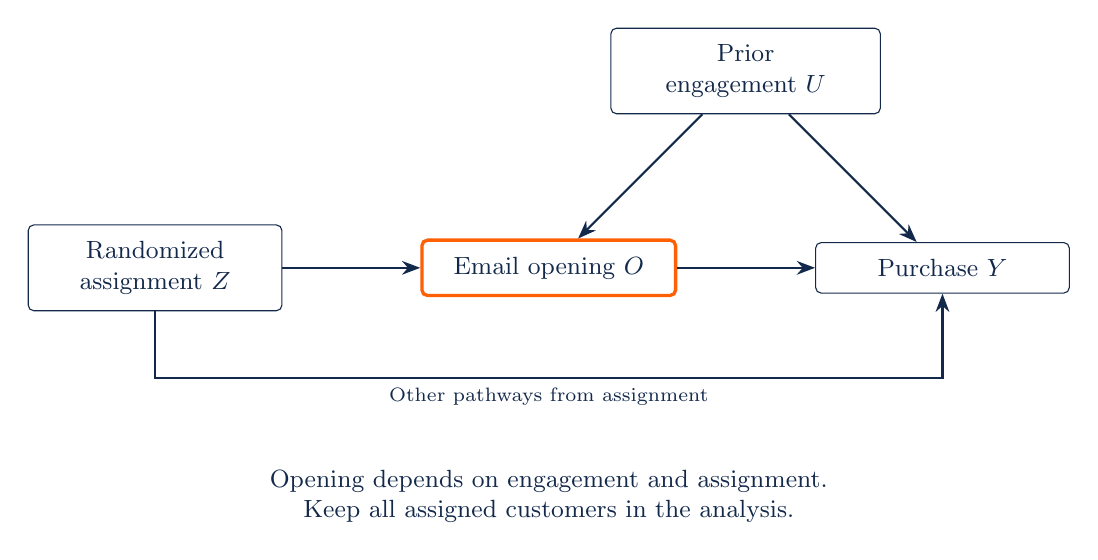
\begin{tikzpicture}
\node[box,text width=2.8cm] (z) at (0,0) {Randomized\\assignment $Z$};
\node[orangebox,text width=2.8cm] (o) at (5,0) {Email opening $O$};
\node[box,text width=2.8cm] (y) at (10,0) {Purchase $Y$};
\node[box,text width=3cm] (u) at (7.5,2.5) {Prior\\engagement $U$};
\draw[edge] (z)--(o);\draw[edge] (o)--(y);\draw[edge] (u)--(o);\draw[edge] (u)--(y);
\draw[edge] (z.south)--(0,-1.4)--node[below,font=\scriptsize] {Other pathways from assignment} (10,-1.4)--(y.south);
\node[align=center,text width=11cm] at (5,-2.9) {Opening depends on engagement and assignment.\\Keep all assigned customers in the analysis.};
\end{tikzpicture}

\end{adjustbox}
\endgroup
\par\medskip
{\small Randomized assignment is distinct from engagement-driven email opening.\par}
\note{Control variables should follow the causal structure and timing. Conditioning on a variable affected by treatment can change the estimand or introduce selection.

M6, Section 6.2, Marketing Analytics Lecture Notes. \url{../06_Lecture_Notes/modules/M06_Causal_Inference_and_Experiments.md}}
\end{frame}
\begin{frame}{Email Assignment and Purchase}
\usebeamercolor[fg]{normal text}
\vfill
\centering
{\small\begin{tabular}{lrrr}
\toprule
Assigned Group & Customers & Purchases & Rate \\
\midrule
Email & 1,000 & 130 & 13\% \\
Control & 1,000 & 100 & 10\% \\
\bottomrule
\end{tabular}}
\par\medskip
Synthetic experiment. Each customer has one binary outcome.
\vfill
\note{The difference is three percentage points. Relative to a 10\% control rate, that equals a 30\% relative increase. The two descriptions use different denominators.

M6, Section 6.4, Marketing Analytics Lecture Notes. \url{../06_Lecture_Notes/modules/M06_Causal_Inference_and_Experiments.md}}
\end{frame}
\begin{frame}{An Assignment-Effect Estimate}
\usebeamercolor[fg]{normal text}
\noindent Compare purchase rates across all assigned customers.
\medskip
\[
\widehat\tau=\frac{130}{1000}-\frac{100}{1000}=0.03
\]
\medskip
\noindent The estimated effect is three additional purchases per 100 assigned customers.
\note{This is an intention-to-treat comparison under the stated randomized design. An opened-email comparison would use a different selected population.

M6, Section 6.4, Marketing Analytics Lecture Notes. \url{../06_Lecture_Notes/modules/M06_Causal_Inference_and_Experiments.md}}
\end{frame}
\begin{frame}{Sampling Uncertainty}
\usebeamercolor[fg]{normal text}
\noindent Use an independent-group approximation for the synthetic binary outcomes.
\medskip
\[
\widehat{\operatorname{SE}}=\sqrt{\frac{.13(.87)}{1000}+\frac{.10(.90)}{1000}}\approx .0143
\]
\medskip
\noindent An approximate 95\% interval is 0.21 to 5.79 percentage points.
\note{The interval uses a large-sample normal approximation and independent customer assignments. It does not include systematic outcome measurement errors or interference.

M6, Section 6.4, Marketing Analytics Lecture Notes. \url{../06_Lecture_Notes/modules/M06_Causal_Inference_and_Experiments.md}}
\end{frame}
\begin{frame}{Contribution and Decision Uncertainty}
\usebeamercolor[fg]{normal text}
\vfill
\begin{slidebullets}
\item An extra purchase contributes 40 dollars.
\item Delivery costs 0.50 dollars per assigned customer.
\item Estimated incremental contribution is 0.70 dollars per customer.
\end{slidebullets}
\vfill
\note{The same transformation of the effect interval gives approximately -0.42 to 1.82 dollars. The calculation assumes no additional discount cost and fixed contribution per additional purchase.

M6, Section 6.4, Marketing Analytics Lecture Notes. \url{../06_Lecture_Notes/modules/M06_Causal_Inference_and_Experiments.md}}
\end{frame}
\begin{frame}[fragile]{The Experiment Calculation}
\usebeamercolor[fg]{normal text}
\noindent Reproduce the effect and its contribution implication.
\begin{lstlisting}
from math import sqrt
p1, p0, n = 0.13, 0.10, 1000
effect = p1 - p0
se = sqrt(p1*(1-p1)/n + p0*(1-p0)/n)
interval = (effect - 1.96*se, effect + 1.96*se)
profit = 40 * effect - 0.50
assert round(profit, 2) == 0.70
\end{lstlisting}
{\small The point estimate is positive while the contribution interval includes losses.\par}
\note{If treatment changes basket size, returns, or margins, purchase incidence alone no longer gives the contribution effect. Measuring contribution directly can better match the decision.

M6, Section 6.4, Marketing Analytics Lecture Notes. \url{../06_Lecture_Notes/modules/M06_Causal_Inference_and_Experiments.md}}
\end{frame}
\begin{frame}{Power Begins With the Useful Effect}
\usebeamercolor[fg]{normal text}
\vfill
\begin{slidebullets}
\item Choose the smallest effect that could change the action.
\item Use the expected outcome variance and assignment unit.
\item Halving the target effect approximately quadruples sample size.
\end{slidebullets}
\vfill
\note{At baseline probability 0.10, a two-point effect, two-sided 5\% level, and 80\% power, a common-variance normal approximation gives 3,528 customers per arm.

M6, Section 6.5, Marketing Analytics Lecture Notes. \url{../06_Lecture_Notes/modules/M06_Causal_Inference_and_Experiments.md}}
\end{frame}
\begin{frame}{Implementation Checks}
\usebeamercolor[fg]{normal text}
\vfill
\begin{slidebullets}
\item Reconcile assigned counts and intended allocation.
\item Check missing outcomes and tracking by assignment.
\item Preserve the planned outcome horizon.
\item Investigate exclusions that depend on treatment response.
\end{slidebullets}
\vfill
\note{A randomization protocol does not prevent differential tracking failures. Sample-ratio discrepancies can reveal implementation problems. Chance covariate imbalance alone does not invalidate a correctly implemented randomization.

M6, Section 6.6, Marketing Analytics Lecture Notes. \url{../06_Lecture_Notes/modules/M06_Causal_Inference_and_Experiments.md}}
\end{frame}
\begin{frame}{Prior Outcomes and Precision}
\usebeamercolor[fg]{normal text}
\noindent Adjust the outcome using a pre-treatment measure $X$.
\medskip
\[
Y_i^{\mathrm{adj}}=Y_i-\theta(X_i-\bar X)
\]
\medskip
\noindent A predictive baseline can reduce residual variation while preserving the assignment comparison.
\note{CUPED uses a pre-treatment covariate and an appropriately specified adjustment. The variance reduction does not create treatment variation or repair selection into treatment.

M6, Section 6.15, Marketing Analytics Lecture Notes. \url{../06_Lecture_Notes/modules/M06_Causal_Inference_and_Experiments.md}}
\end{frame}
\begin{frame}{mHealth Baseline Activity Improves Precision}
\usebeamercolor[fg]{normal text}
\centering
\begingroup
\begin{adjustbox}{max width=0.98\textwidth,max totalheight=0.65\textheight}
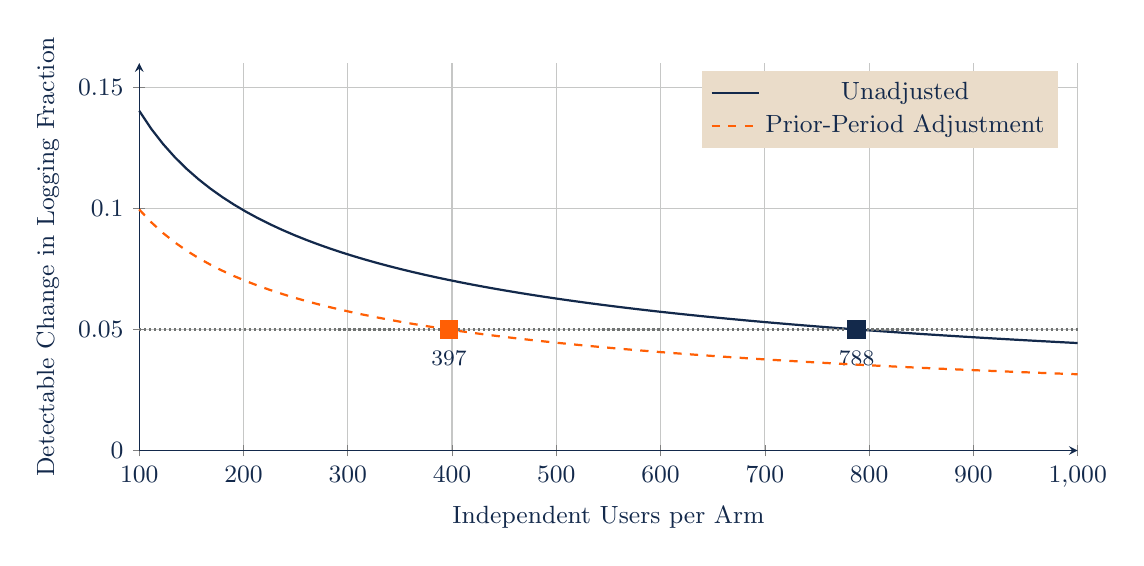
\begin{tikzpicture}
\begin{axis}[xlabel={Independent Users per Arm},ylabel={Detectable Change in Logging Fraction},xmin=100,xmax=1000,ymin=0,ymax=.16,ytick={0,.05,.10,.15},yticklabel style={/pgf/number format/fixed,/pgf/number format/precision=2},grid=major,legend style={at={(.98,.98)},anchor=north east}]
\addplot[IlliniBlue,solid,domain=100:1000,samples=80] {sqrt(2*0.1254625200*(1.959963985+0.841621234)^2/x)};
\addlegendentry{Unadjusted}
\addplot[only marks,IlliniBlue,mark=square*,mark size=3pt,forget plot] coordinates {(788,.05)};
\node[anchor=north,font=\footnotesize] at (axis cs:788,.045) {788};
\addplot[IlliniOrange,dashed,domain=100:1000,samples=80] {sqrt(2*0.0631502639*(1.959963985+0.841621234)^2/x)};
\addlegendentry{Prior-Period Adjustment}
\addplot[only marks,IlliniOrange,mark=square*,mark size=3pt,forget plot] coordinates {(397,.05)};
\node[anchor=north,font=\footnotesize] at (axis cs:397,.045) {397};
\addplot[Storm,densely dotted,forget plot] coordinates {(100,.05)(1000,.05)};
\end{axis}\end{tikzpicture}

\end{adjustbox}
\endgroup
\par\medskip
{\small Planning calculation uses historical user-level variance and a five-point target.\par}
\note{These are power-planning implications of observed historical variances, not a realized intervention effect. The future population, outcome process, and assignment need to match the planning conditions.

M6, Section 6.15, Marketing Analytics Lecture Notes. \url{../06_Lecture_Notes/modules/M06_Causal_Inference_and_Experiments.md}}
\end{frame}
\begin{frame}{Model and Library Contributions}
\usebeamercolor[fg]{normal text}
\centering
\begingroup
\begin{adjustbox}{max width=0.98\textwidth,max totalheight=0.65\textheight}
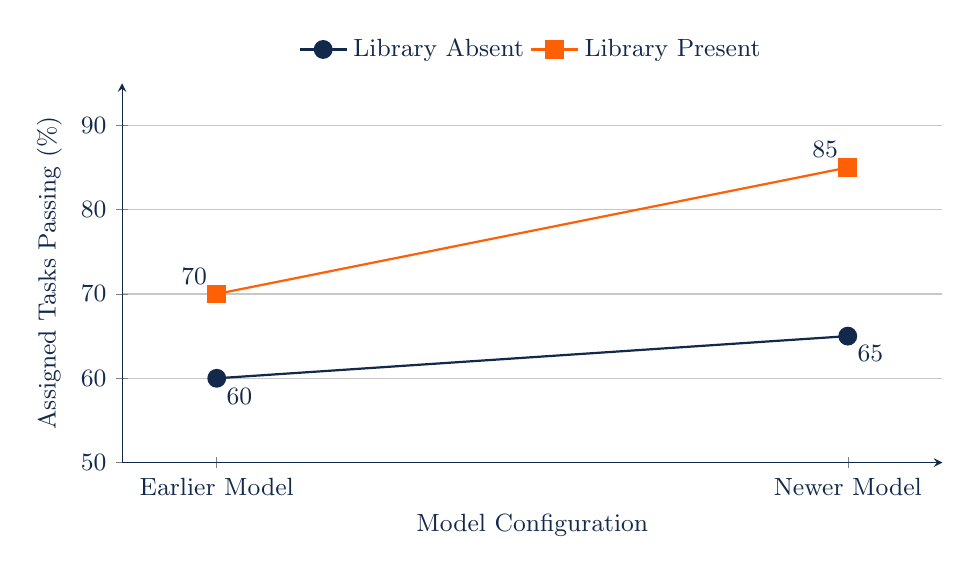
\begin{tikzpicture}
\begin{axis}[width=12cm,height=6.4cm,xmin=-.15,xmax=1.15,ymin=50,ymax=95,
xtick={0,1},xticklabels={Earlier Model,Newer Model},ytick={50,60,70,80,90},
ylabel={Assigned Tasks Passing (\%)},xlabel={Model Configuration},ymajorgrids=true,
legend style={at={(.5,1.03)},anchor=south,legend columns=2,fill=none}]
\addplot[IlliniBlue,mark=*,mark size=3pt] coordinates {(0,60) (1,65)};
\addlegendentry{Library Absent}
\addplot[IlliniOrange,mark=square*,mark size=3pt] coordinates {(0,70) (1,85)};
\addlegendentry{Library Present}
\node[anchor=north west] at (axis cs:0,60) {60};
\node[anchor=north west] at (axis cs:1,65) {65};
\node[anchor=south east] at (axis cs:0,70) {70};
\node[anchor=south east] at (axis cs:1,85) {85};
\end{axis}
\end{tikzpicture}

\end{adjustbox}
\endgroup
\par\medskip
{\small Synthetic counts: 100 assigned tasks per condition; common rubric and resource limits.\par}
\note{The interaction is ten percentage points. Moving from the initial condition to the newer model with the library improves the imposed rate by twenty-five points. Independent assignments, valid reference outcomes, and fresh tasks would be required for an empirical causal comparison. These counts are constructed, with unfinished tasks counted as failures.

Marketing Analytics Lecture Notes, M6 §6.19.}
\end{frame}
\begin{frame}[fragile]{An Interaction Calculation}
\usebeamercolor[fg]{normal text}
\noindent The four rates are imposed teaching inputs.
\begin{lstlisting}
q00, q01, q10, q11 = 0.60, 0.70, 0.65, 0.85
model_alone = q10 - q00
library_after_model = q11 - q10
interaction = (q11-q10) - (q01-q00)
assert round(interaction, 2) == 0.10
assert round(model_alone + library_after_model, 2) == 0.25
\end{lstlisting}
{\small A joint gain does not uniquely allocate the interaction to either component.\par}
\note{Run factorial.py to reproduce both paths to the joint change using exact rational arithmetic. Randomize at the team or project level when outputs share personnel, prompts, or helper code. Record actual cost alongside pass rates and resource ceilings.

M6 §6.19. \url{../03_Data_and_Code/AI_Workflows/factorial.py}}
\end{frame}
\begin{frame}{Coding Exercise: An Experiment Plan}
\usebeamercolor[fg]{normal text}
\vfill
\begin{slidebullets}
\item Compute the factorial contrasts alongside the email effect.
\item Change contribution, delivery cost, and the target effect.
\item Specify an mHealth recommendation assignment with a fixed user denominator.
\end{slidebullets}
\vfill
\note{Run ../03\_Data\_and\_Code/Lecture\_Examples/session\_examples.py S09. The mHealth experiment-planning scripts use historical variation and an explicitly simulated zero-effect assignment. Their output must remain labeled as planning and simulation. The AI\_Workflows folder supplies complete standard-library calculations with synthetic inputs.

M6, Section 6.13, Marketing Analytics Lecture Notes. \url{../06_Lecture_Notes/modules/M06_Causal_Inference_and_Experiments.md}}
\end{frame}
\begin{frame}{Interference and Assignment Units}
\usebeamercolor[fg]{normal text}
\vfill
\begin{slidebullets}
\item Customers can share offers or affect one another.
\item Stores can divert purchases from nearby locations.
\item The assignment unit should reflect the likely spillovers.
\end{slidebullets}
\vfill
\note{If one treated store gains by taking business from a comparison store, the store-level difference can exceed the chain-wide gain. Cluster assignment changes both interpretation and precision.

M6, Section 6.10, Marketing Analytics Lecture Notes. \url{../06_Lecture_Notes/modules/M06_Causal_Inference_and_Experiments.md}}
\end{frame}
\begin{frame}{A Treatment Arm Needs a Defensible Design}
\usebeamercolor[fg]{normal text}
\vfill
\begin{slidebullets}
\item Random assignment identifies a comparison.
\item The content of each treatment still affects the customers who receive it.
\item Include customer outcomes, refusal, and stopping conditions.
\end{slidebullets}
\vfill
\note{Randomization does not establish that a deceptive or harmful interface is acceptable. Separate analytical identification from the substantive and regulatory evaluation of each proposed treatment.

ETHICS\_AND\_REGULATION.md, M6.}
\end{frame}
\begin{frame}{Follow Purchases Through Returns}
\usebeamercolor[fg]{normal text}
\vfill
\begin{slidebullets}
\item Pressure and self-assurance can produce different purchase and return patterns.
\item Prespecify the eligible population and both outcome horizons.
\item For cancellation, measure intent, completion, and subsequent charges.
\end{slidebullets}
\vfill
\note{The verified abstract of the randomized online-retailing study reports stronger purchase responses alongside more returns under pressure nudges. Its full text remains unavailable in the collection. The directional result motivates balanced outcomes; exact effects and implementation details require the complete paper. A cancellation study should define eligibility at the initial request and compare lawful designs. See M6 Section 6.20.

\url{https://doi.org/10.1177/00222437231180494}}
\end{frame}
\begin{frame}{From Experiments to Generative Decisions}
\usebeamercolor[fg]{normal text}
\vfill
\begin{slidebullets}
\item Within-campaign comparisons can supervise a model that proposes new messages.
\item The learned ranking inherits the outcome used to define success.
\item Evaluate new proposals in their deployment setting.
\end{slidebullets}
\vfill
\note{Angelopoulos, Lee, and Misra train a language-model improver using historical experimental comparisons. The causal interpretation is tied to the randomized comparison and measured outcome. Transfer to new content requires new evidence.

\url{https://leekevin.io/caLM.pdf}}
\end{frame}
\begin{frame}{Human Review and Customer Evidence}
\usebeamercolor[fg]{normal text}
\vfill
\begin{slidebullets}
\item Check factual claims and consequential terms before deployment.
\item Record customer understanding and the ability to refuse.
\item A robust commercial payoff still requires a justified objective.
\end{slidebullets}
\vfill
\note{Causal Alignment includes human selection and acceptability checks. Their existence is material to a fair critique; their coverage remains a substantive question. Farrell, Korganbekova, and Misra address robustness to a changed deployment distribution, with a selected payoff.

\url{https://leekevin.io/caLM.pdf} \url{https://arxiv.org/abs/2609.07633}}
\end{frame}
\begin{frame}{Experiment Discussion}
\usebeamercolor[fg]{normal text}
\vfill
\begin{slidebullets}
\item Would a conversion gain cover the campaign cost?
\item What changes if only email openers enter the analysis?
\item Which guardrail outcome could reverse the rollout decision?
\end{slidebullets}
\vfill
\note{Contribution uncertainty remains consequential even with a positive purchase effect. Returns, satisfaction, and service burden can alter the decision. The outcome set should reflect the intervention.

M6, Section 6.11, Marketing Analytics Lecture Notes. \url{../06_Lecture_Notes/modules/M06_Causal_Inference_and_Experiments.md}}
\end{frame}
\end{document}
